\externaldocument{../main.tex}

In the previous section I took some shortcuts to give a clearer view of the core components of the
6G architecture while highlighting the idea that the future of mobile communication technologies,
while revolutionary for many different reasons, is just a different spin of an architecture that has
already been proven to be working which is the Cloud infrastructure. It's now time to look under the
rug and explore the problems and some potential solutions that have been proposed.

Since most of the solutions are pretty much interchangeable or work together to solve the same
problems I will first explore the single problems and then move to explaining the various solutions
that have been found, if possible with references to some specific techniques that have been
explored in the literature.

The first problem that needs solving is a model size.

If we consider the network architecture introduced in the last section the network nodes will be
partitioned based on their computational power into the different tiers. If we need to place the
different LLMs based on the need of the various users in the network we now need to take into
consideration two different factors:
\begin{itemize}
	\item The latency: we can put all of the big models (like GPT-4, Stable diffusion, LLaMa,
	      etc...) at the end of the network, while keeping lighter models like (LLaMa7B) closer to the
	      user. Having such an organization would in turn mean that the end users, to get better
	      results, would need to wait for a time that is proportional to the quality of the response.

	      Clearly, if a response from a model like GPT-4v is required then it will be associated with
	      a very big latency due to how big of a leap inside the architecture the message is going to
	      need to do:
	      \begin{itemize}
		      \item Sending the request from END to CLOUD
		      \item Waiting for the request to be processed and the inference to be made
		      \item Sending the response from CLOUD to END
	      \end{itemize}
	      Since the operation of inference is already costly it's much better to be able to do
	      inference (even on bigger models) as close to the edge of the network as possible.

	\item The space and compute: having to load models in memory or even saving them is
	      extremely expensive, that is because of the amount of resources required.
	      As can be seen in \cite{hug-optimization} the dimensions of required VRAM in GPU for LLMs at
	      different ranges of performance (from GPT-3 to bigcoder/starcoder) require between 350 and
	      30 GB of VRAM, which is already extreme for any computing device that might inhabit the Fog.

	      Even the requirements in terms of basic storage are completely out of the capabilities of
	      the majority of devices inside the Fog (175 GB for GPT-3 is a lot, especially if we consider
	      that the user might not have stored locally just the one LLM but might employ different ones
	      for different pourposes).

	      Last but not least, doing inference on the model or training the model will most likely
	      require more compute power than the one available to most of the devices in the Fog.
\end{itemize}

It's clear enough that what is required here is to have a caching system that can allow to train or
re-train the models when needed, while being able to save more than one model on board in order to
serve END devices as fast as possible when necessary. To make matters worse, when doing a re-train
to serve a certain user the task should be done as securely as possible, therefore users' data
cannot be sent through the network to head to a certain node that is responsible for the retraining
procedure.
The safety hazard should be taken with the utmost caution since we are not talking about common data
most of the time, we are talking about training e-health models and such, having any company store
such data for a network re-train should be considered a serious concern and should be avoided at all costs.

SPLIT LEARNING
Split learning (SL) is the first solution that we offer and can solve both problems at the same time.
SL reduces the model size in order to allow for an efficient and secure training process, by
splitting the model in two parts, the smaller one will be living on the END device, while the bigger
one will be living on the CONTROLLER. The technique is clearly recursive and therefore the same
conclusions can be drawn if a model is too big to reside inside the CONTROLLER.

SL is a really powerful tool going forward since it allows the model to be fine-tuned to the user's
preference without having to send very private data to servers. That can be done by dividing the
learning process and allowing devices in the END to handle the part of the training that has to do
with the user's data, while the closest CONTROLLER (or the any CLOUD server) handles the training of
the general pourpose part. The whole training process only requires the exchange of intermidiate
gradient computations as shown in the picture below:
\begin{figure}
	\center
	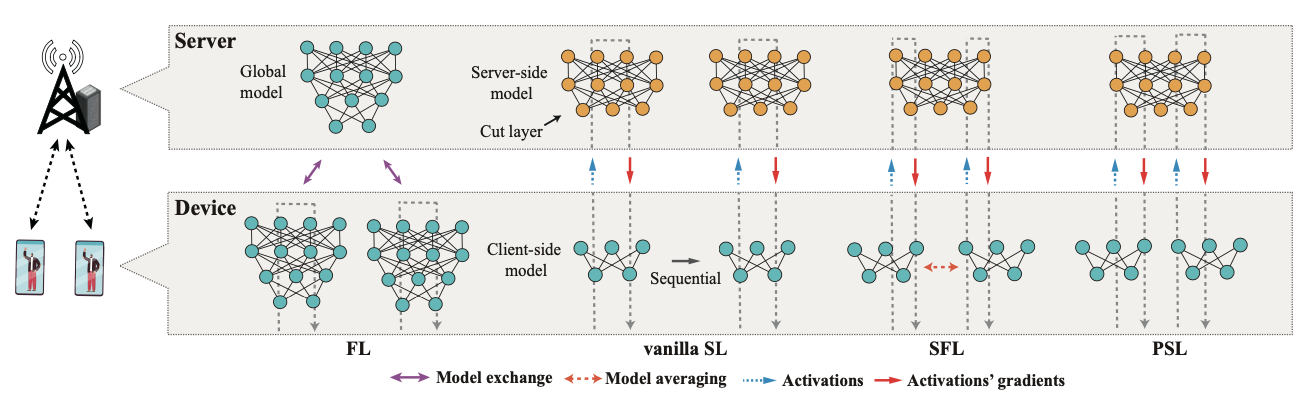
\includegraphics[scale=0.65]{figures/split-learning.png}
	\caption{An example of the structure of a network implementing SL for model trainig
		\cite{split-learning}}
\end{figure}

FEDERATED LEARNING

EFFICIENT TUNING
